%!TEX root = ../main.tex
\section{Augmenting path algorithms}
\subsection{Introduction}
The idea behind the augmenting path algorithms is as follows : 
As long as there is a path from the source to the sink, we send flow along this path. And so on until there is no more path from the source to the sink. \newline

An available path from the source to the sink is called \textit{augmenting path} and to find it, we use the \textit{residual graph}. A \textit{residual graph} is a double oriented graph with the available capacities. For instance here is a graph with its \textit{residual graph}: \newline

\begin{figure}[!h]
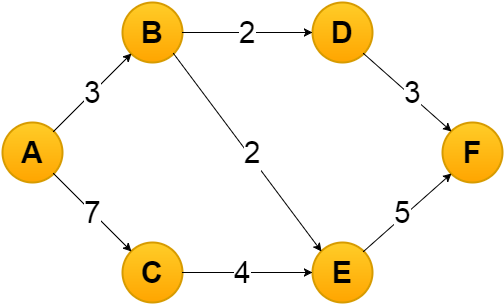
\includegraphics[width=7.5cm,height=4.5cm]{images/graph.png}\hfill
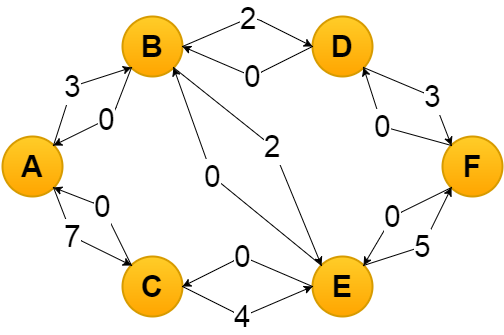
\includegraphics[width=7.5cm,height=4.5cm]{images/residualgraph.png}
\caption{A graph with its residual graph}
\end{figure}


When an \textit{augmenting path} is found, we send a flow equivalent to the minimum capacity of the edges of this path. We update the \textit{residual graph} by decreasing capacities in forward edges and increasing capacities in backward edges. Then we look for a new augmenting path. \newline

Here is the \textit{residual graph} after sending 4 units of flow through the \textit{augmenting path} A-C-E-F : \newline

\begin{center}
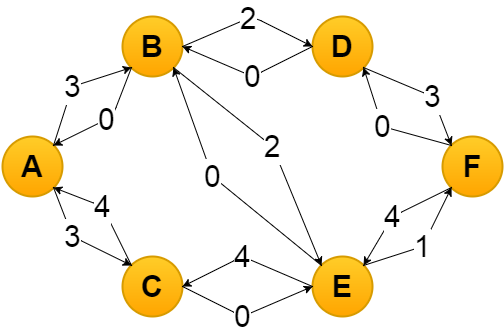
\includegraphics[width=7.5cm,height=4.5cm]{images/residualgraph2.png}
\captionof{figure}{Residual graph}
\end{center}

The pseudo-code of the augmenting path algorithm is given here :

\begin{algorithm}[h]

 Look for an augmenting path\;
 \While{There is an augmenting path}{
  Send flow through this path\;
  Update the residual graph\;
  Look for an new augmenting path\;
 }
\end{algorithm}

\subsection{Ford-Fulkerson and Edmonds-Karp}
There are two main augmenting path algorithms, Ford-Fulkerson (published in 1956) and Edmonds-Karp (published in 1972). The second being a variant of the first one. Indeed, the unique difference between both is the way of looking for an \textit{augmenting path} in the \textit{residual graph}. \newline

Ford-Fulkerson uses a depth-first search while Edmonds-Karp uses a breadth-first search.



\subsection{Complexities}
The max flow problem, being a problem of complexity class P, can be solved at polynomial time. When the capacities are integers, Ford-Fulkerson is bounded by $O(E*f)$ and Edmonds-Karp by $O(V*E^2)$, where $E$ is the number of edges in the graph, $V$ is the number of vertices and $f$ is the maximum flow.

\begin{description}
\item[Ford-Fulkerson]{is in $O(E*f)$ because each augmenting path can be found in $O(E)$ and in the worst case, the flow will increase by 1.}
\item[Edmonds-Karp]{is in $O(V*E^2)$ because the breadth-first search assures us that after each iteration, the length of the augmenting path can't decrease. Futhermore, the length of the augmenting path can stay the same for at most $E$ iterations before increasing. We also know that the length of the augmenting path is between $1$ and $V-1$. Thus there are at most $V*E$ iterations and each augmenting path can be found in $O(E)$.}
\end{description}


\section{Pre-flow algorithms}
